\documentclass[colorlinks=true,pdfstartview=FitV,linkcolor=blue,
            citecolor=red,urlcolor=magenta]{ligodoc}

\usepackage{graphicx}
\usepackage{amssymb}
\usepackage{amsmath}
\usepackage{longtable}
\usepackage{rotating}
\usepackage[usenames,dvipsnames]{color}
\usepackage{fancyhdr}
\usepackage{subfigure}
\usepackage{hyperref}
\ligodccnumber{T}{19}{00287}{}{v1}% \ligodistribution{AIC, ISC}


\title{Data Clustering Techniques for the Correlation of Environmental Noise to Signals in LIGO Detectors}

\author{Jacob Bernhardt, Anamaria Effler, Rana Adhikari}

\begin{document}

\section{Introduction}
The LIGO project uses laser interferometry to measure gravitational waves (GWs).
LIGO interferometers transduce their relative arm length differences caused by GWs to a signal composed of optical power, known as DARM.
Due to the amplitude scales of astrophysical GWs, The LIGO detectors have to operate at a very high sensitivity; the spectral density of a measurable length difference is as low as $2\times 10^{-20}~\mathrm{m}/\sqrt{\mathrm{Hz}}$ at 100 Hz.
The design of earthbound LIGO is thus heavily focused on the filtering and isolation of environmental noise.

To help identify and characterize environment-based noise, the LIGO detector has a Physical Environment Monitoring (PEM) system, a diverse array of environmental sensors positioned all over the facility\cite{aepaper}.
This is used for a multitude of purposes, including the data quality report (DQR) used for time segment vetoing, based on direct coherence of PEM channels to DARM.
Supplementing coincidence analysis between the two detectors, DQR prevents GW-like noise transients from being falsely categorized as events.
Thus, detector livetime can be increased by figuring out how to decouple environmental noise from DARM.
Directly coupling noise, found by basic coherence, has been already addressed, but the complexity of the detector causes many noise sources to up- or down-convert.
These require some more careful statistical correlation to identify, and are sometimes not well understood.
\begin{figure}
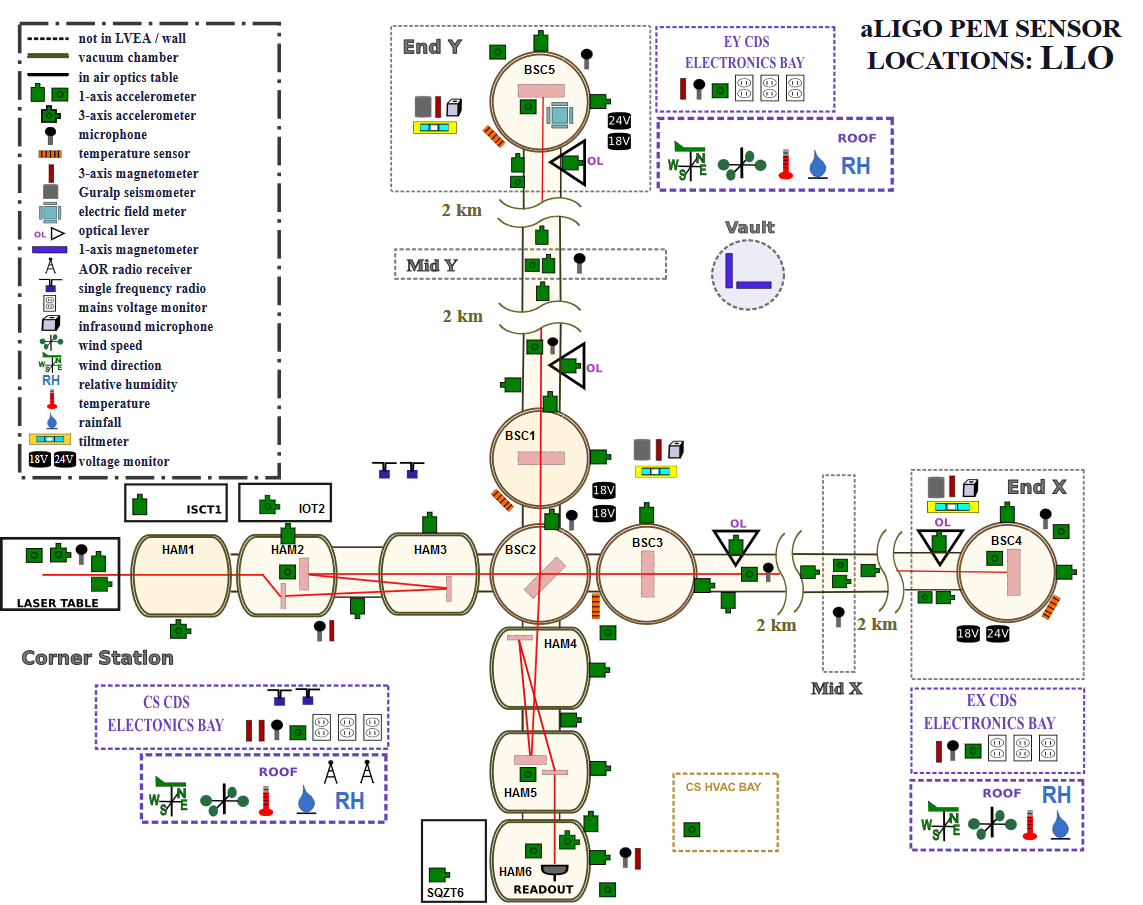
\includegraphics[width=\textwidth]{assets/llopem.png}
\caption{Schematic PEM map at the LIGO Livingston Observatory (L1). Shaded areas are in vacuum.}
\end{figure}
\begin{figure}
  \begin{minipage}[c]{0.67\textwidth}
  \begin{tabular}{c}
  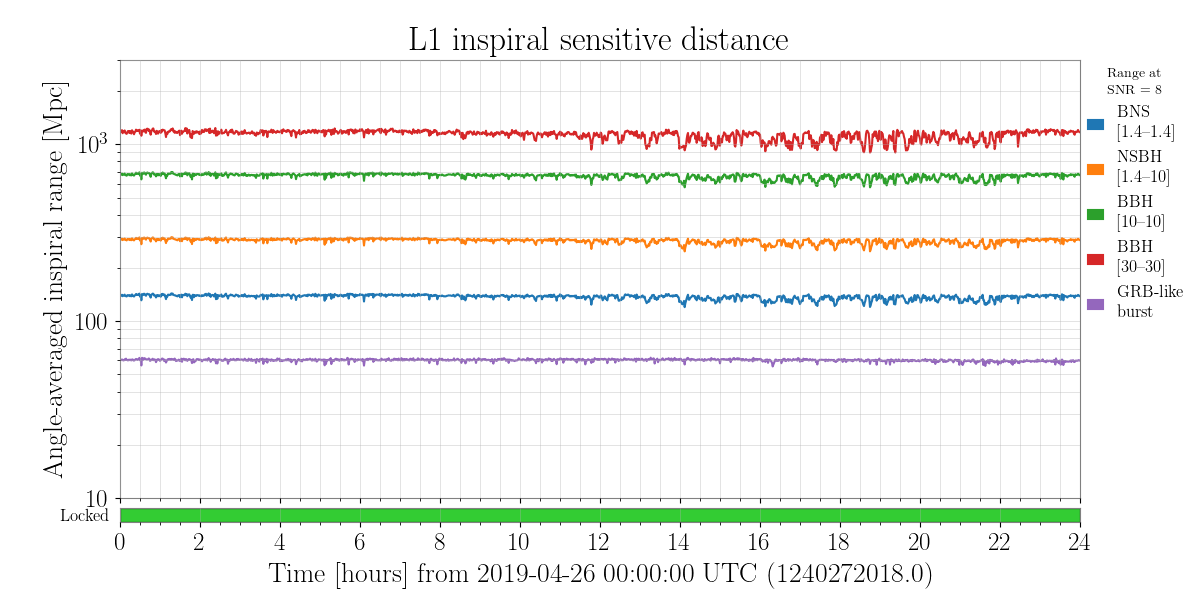
\includegraphics[width=\textwidth]{assets/L1-LOCKED_216737_RANGE-1240272018-86400.png}   \\  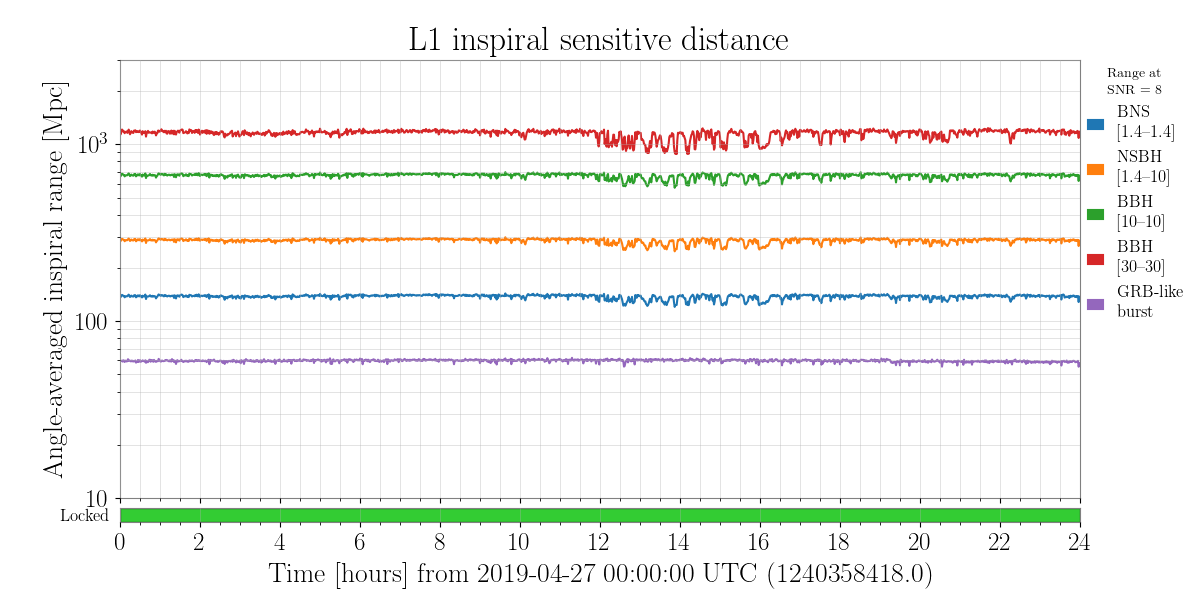
\includegraphics[width=\textwidth]{assets/L1-LOCKED_216737_RANGE-1240358418-86400.png}
  \end{tabular}
  \end{minipage}\hfill
  \begin{minipage}[t]{0.3\textwidth}
    \caption{Detector range at L1 seems to consistently reduce during the day ($\sim$6am-5pm CST). For large BBH in these plots, the reduction is about 300 Mpc. The source of this has been pinpointed to the Y end station, but the mechanism isn't fully clear.}
  \end{minipage}
\end{figure}

Separating noise sources out of a signal can be considered a clustering problem in a space covering different frequency bands in which noise appears.
A previous LIGO SURF student has evaluated several data clustering algorithms with respect to their ability to properly sort out frequency elements of seismometer signals caused by specific earthquake events\cite{roxana}.
Both the $k$-means algorithm, which aims to make clusters with low standard deviation, and the DBSCAN algorithm, which minimizes overall inter-point distance in clusters, were evaluated using multiple methods, including the Calinsky-Harabaz  index and direct comparison to earthquake times via time labeling of points, ultimately showing poor earthquake identification.
A long short-term memory (LSTM) recurrent neural network (RNN) seemed to work much better, but due to small input sample size, this solution may have been be plagued by over-fitting.
Thus, it is imperative that a more robust frequency clustering mechanism be designed for the PEM system.

\section{Objectives}
% What do you aim to accomplish in your project? What will you measure, and under what conditions; or, what will you calculate, model, or simulate; or what will you design, and what are the requirements; or what will you build or test? What is your starting point? What are your initial assumptions or conditions? What will be the result or product of a successful outcome for your project? What are the criteria for project completion or for success? (In other words, how will you know when you have accomplished what you set out to do?)
\begin{itemize}
\item
As a primary goal, \textbf{algorithms or clustering approaches which correctly identify known noise events need to be found}.
As every algorithm has inbuilt assumptions about the dataset it is applied to, the results of an algorithm performance test on labeled data will yield information about the structure of the data.
The general temporal non-stationarity of the DARM noise will need to be accounted for by varying testing time windows.
\item
The secondary goal is to \textbf{create a clustering approach to discover previously unknown noise correlations and possibly sources}.
This is where the ``detector characterization tool'' that this project aims to advance will be functional---revealing new noise coupling pathways will help identify ways to improve the detector sensitivity.
\end{itemize}

\section{Approach}
% Specifically, how will you reach your objective or produce your desired final product? What are the principal steps or milestones along the path? How long will each take? What steps promise to be the most difficult, and how will you overcome the difficulties? What equipment or other resources will you need? Which of these are inherited, and which will you have to make or procure? With what other people or groups will you be collaborating? Will completion of your project depend on results from other people in related projects? (That question may be especially pertinent for team projects.)

Initially, a program will be written to take the spectral power of any PEM channel, in the form of band-limited RMS (BLRMS), likely using established methods like looping through a smoothed spectogram of the channel\cite{vajente}.

To reach the first objective, a modular \texttt{python} testing suite will be written to probe the structure of the multidimensional frequency-domain sensor data.
This will strategically implement \texttt{scikit-learn} clustering algorithms and classifiers with different optimal regimes of function or working assumptions and evaluate them using point labeling. 
This will require, additionally to researching clustering or unsupervised classification algorithms, thinking of as many variables which may affect the data structure (such as looking at different time windows) and intelligently testing them. 
Optimizations will need to be considered so that run times are reasonable.

The program tackling the second objective will use working clustering approaches identified in the first objective to find new noise correlations.
In the event that no individual algorithm or technique outperforms the rest for all types of sensory data, the final program will use the modular programming environment created for the testing suite to match techniques to the regimes that they work in.
The structure of the input data as determined by the first objective, including the dimensionality probed by the extra variables, may lend itself to additional algorithms that can be used to combine the target regimes.
To this end, extra algorithm research will be conducted with specific consideration of the solved structure.

%%% Local Variables:
%%% mode: latex
%%% TeX-master: "../proposal"
%%% End:


\section{Project Schedule}
% Preparing a schedule of the principal activities and events is a good way of showing the readers that you have taken a systematic approach to planning your work.
\paragraph{Before Arrival}
\begin{itemize}
\item Research algorithms to use
\item Develop glitch-resistant BLRMS-making code
\item Continue familiarizing with \texttt{scikit-learn} by adapting old clustering code for beamtube accelerometers
\end{itemize}
\paragraph{Week 1-2}
\begin{itemize}
\item Familiarize with types of PEM data that can have labeled events
\item Complete the algorithm testing suite
\end{itemize}
\paragraph{Week 3-4}
\begin{itemize}
\item Develop ways to plug channels into the suite
\item Run suite on determined variety of channel combinations and regimes
\end{itemize}
\paragraph{Week 5-6}
\begin{itemize}
\item Examine results, decide next steps
\item Research new algorithms
\item Adapt initial codebase for application
\end{itemize}
\paragraph{Week 7-8}
\begin{itemize}
\item Try to reveal new PEM-DARM coupling mechanisms and propose/implement solutions
\end{itemize}
\paragraph{Week 9-10}
\begin{itemize}
\item Finish up final analysis and writing final report.
\end{itemize}

\begin{thebibliography}{2}
\bibitem{aepaper} A. Effler, R. M. S. Schofield, V. V. Frolov, G. Gonz{\'{a}}lez, K. Kawabe, J. R. Smith, J. Birch, and R. McCarthy, Classical and Quantum Gravity \textbf{32}, 035017 (2015).
\bibitem{roxana} LIGO Document T1700198-v1
\bibitem{vajente} aLIGO LLO Logbook entry 45374 by Gabriele Vajente
\end{thebibliography}



\end{document}
